\chapter{Architectuur}

\section{Architecturale beslissingen}
Zoals beschreven in vorige secties gaan we een library ontwikkelen om applicaties te kunnen monitoren. Tracklytics is de naam van de library en wordt in het vervolg van dit document gebruikt om de library aan te duiden. \\
In deze sectie worden de architecturale beslissingen die gemaakt zijn uit de doeken gedaan. Aan de hand van diagrammen wordt besproken hoe Tracklytics conceptueel werkt. \\


Tracklytics bestaat uit volgende hoofdcomponenten:
\begin{itemize}
\item UserApplication: De applicatie die de developer wil monitoren
\item TracklyticsCore: De Tracklytics library die in de applicatie verwerkt is.
\item TracklyticsBackend: De backend die de informatie verwerkt die van de TracklyticsCore komt.
\item Dashboard: Een dashboard om alle informatie weer te geven.
\end{itemize}

\begin{figure}[!h]
  \centering
  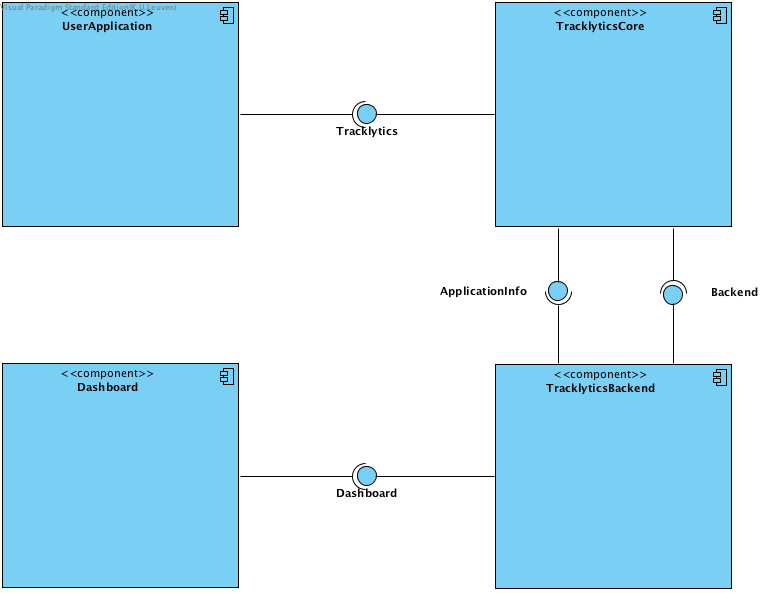
\includegraphics[scale=0.4]{Afbeeldingen/Architectuur/Component}
  \caption{Component diagram Tracklytics library.}
  \label{fig:component}
\end{figure}

\begin{figure}[!h]
  \centering
  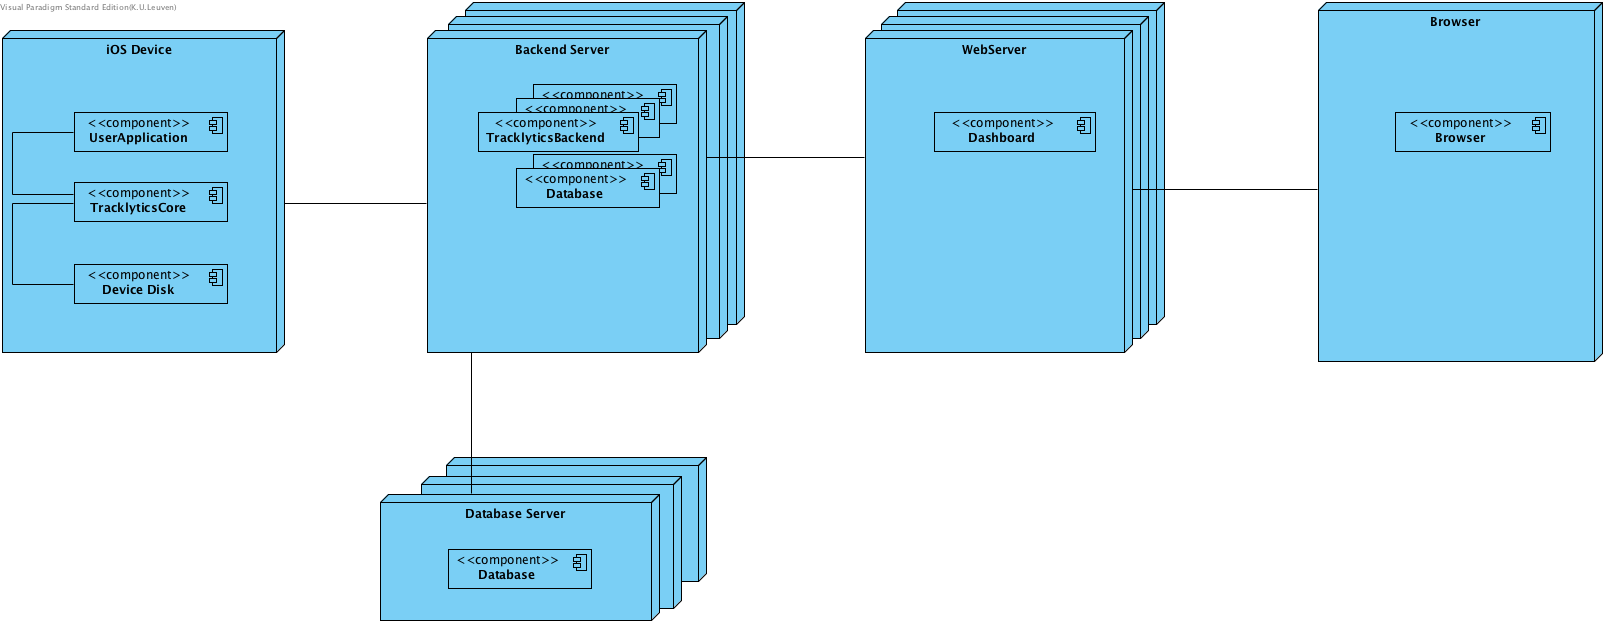
\includegraphics[scale=0.30]{Afbeeldingen/Architectuur/Deployment}
  \caption{Deployment diagram Tracklytics library.}
  \label{fig:deployment}
\end{figure}

\subsection{Deployment Diagram}
Het deployment diagram toont op welke nodes de componenten draaien. Zoals je kan zien draait de UserApplication en de TracklyticsCore op het toestel van de gebruiker zelf (een iOS device). De TracklyticsBackend draait op een backend server die gerepliceerd kan worden. Deze staat in verbinding met een Database server waar alle data wordt opgeslagen. Het Dashboard draait op een webserver. Deze staat in verbinding met de backend server om de data te kunnen ophalen.

\subsection{Component Diagram}
Het component diagram \ref{fig:component} duidt aan welke componenten een rol spelen in het bouwen van de Tracklytics library. In de volgende secties worden de verschillende componenten beschreven en hun rol wordt uitgelegd.


\subsubsection{UserApplication}
De UserApplication component bestaat uit de applicatie ontwikkeld door de developers. Deze verschilt per applicatie. De UserApplication stuurt data door naar de TracklyticsCore component via de Tracklytics interface. De interface wordt in de volgende sectie besproken. De developers kiezen zelf welke elementen getrackt en gemonitord worden. Deze component draait op het toestel van de gebruiker.

\subsubsection{TracklyticsCore}
\paragraph{Monitoring}
De TracklyticsCore component stelt de library voor die in deze thesis ontwikkeld wordt. De component draait op het toestel van de gebruiker. De TracklyticsCore component verzamelt informatie die hij doorkrijgt van de UserApplication component, slaat deze tijdelijk op het toestel op om deze dan later door te sturen naar de TracklyticsBackend component via de Backend interface. Deze interface wordt in de volgende sectie besproken.

De TracklyticsCore component biedt een Tracklytics interface aan. De UserApplication kan deze interface gebruiken om data te verzamelen. De TracklyticsCore stuurt deze later naar de server zoals besproken wordt in volgende sectie.\\

De interface bestaat uit het gebruik van 5 elementen, namelijk:
\begin{itemize}
\item Counter
\item Meter
\item Histogram
\item Timer
\item Gauge
\end{itemize}

Deze elementen worden verder besproken in het hoofdstuk over het klassediagram \ref{sec:Klassediagram}.\\

\paragraph{Data availability}
Smartphones vallen weleens zonder internet connectiviteit. Tracklytics zend de data over het internet naar de backend om deze op te slaan in een database. Als de internetverbinding zou wegvallen, dan zou er mogelijks belangrijke data verloren gaan. Om dit scenario te voorkomen slaan we de data tijdelijk op op de harde schijf van de telefoon. Indien de smartphone dan terug verbinding met het internet heeft gemaakt kan de data alsnog gesynchroniseert worden met de backend. De data wordt tijdelijk opgeslagen, dus nadat de data gesynchroniseerd is wordt deze van de smartphone verwijderd. 

\paragraph{On Demand}
Het is de bedoeling de developer zoveel mogelijk vrijheid te geven in het monitoren van de applicatie. Om deze vrijheid te verhogen voegen we het On Demand aan- of uitzetten van het monitoren toe aan Tracklytics. Een developer kan vanuit het dashboard aangeven of de applicatie gemonitord moet worden of niet. Dit kan gebruikt worden om op de piekdagen of piekmomenten het monitoren aan te zetten. Zo kan uitgezocht worden of er een bottleneck bestaat als het gebruik van de applicatie piekt. \\
Indien een developer ontdekt dat er geen bottleneck of problemen zijn met de app en deze niet verder gemonitord moet worden, dan is het handig om de monitoring uit te kunnen zetten. Dit zorgt ook voor een prestatieboost, omdat er niet meer gesynchroniseerd moet worden naar de server en de data moet niet meer op het toestel verwerkt en opgeslagen worden door Tracklytics.


\paragraph{Aggregatie}
De data die doorgestuurd wordt naar de server zegt op zichzelf niets. Om een goede analyse weer te geven in het dashboard moet deze data geaggregeerd worden. Er zijn twee plaatsen waar deze aggregatie uitgevoerd kan worden, namelijk op de smartphone zelf in de Tracklytics library of in de backend. \\
De reden om de aggregatie op de smartphone uit te voeren is dat er zo minder data gecollecteerd moet worden in de backend om de data visueel voor te stellen. Er is dus een prestatiewinst om de aggregatie op de smartphone uit te voeren. 
Een nadeel is dat deze aggregatie meer CPU tijd van de smartphone gebruikt dan als we de aggregatie in de backend uitvoeren. Er is dus een goede afweging nodig waar deze aggregatie gebeurt.\\

Een functie in het dashboard zou ervoor kunnen zorgen dat de developer de optie krijgt om te kiezen of deze aggregatie op de telefoon of in de backend uit te voeren. Dit geeft de developer ook weer meer vrijheid om deze keuzes te maken.

\paragraph{AB Testing}
AB testing is een mechanisme dat grote bedrijven, zoals facebook, gebruiken om nieuwe features uit te rollen naar de gebruikers. Het mechanisme werkt als volgt: er bestaat een versie A en een versie B van de software met B de nieuwere versie. AB testing zorgt ervoor dat de uitrol van de versie B geleidelijk verloopt. De gebruikers van de software worden dus in twee (of meerdere) groepen opgedeeld door een eigenschap. Deze eigenschap kan vanalles zijn, namelijk: geografische locatie, ingestelde taal, de gebruikte browser, het type toestel, enz. Indien er dan een probleem met versie B is, dan bestaat dit enkel bij de groep die versie B al verkregen is en dus niet bij alle gebruikers. Hierdoor merkt enkel die groep dat er een probleem is en kan versie B aangepast worden om dit probleem op te lossen of eventueel kan ervoor gezorgd worden dat iedereen terug versie A gebruikt. \\

In mobiele applicaties is het moeilijker om echt aan AB testing te doen, omdat deze applicaties meestal statisch zijn, er moet een update in de app store komen om een nieuwe versie uit te rollen. Dit staat pal tegenover websites die hun webpaginas van een server halen en dus bij elk vernieuwen van een webpagina helemaal anders zijn. 
Een workaround van dit probleem is dat de mobiele applicatie de code van de nieuwe versie al bevat en ook nog de oude code erin heeft staan. Tracklytics kan dan een functie in het dashboard aanbieden om de groepen op te delen in twee (of meerdere) groepen op basis van eigenschappen die de developer kan kiezen. In de mobiele applicatie moeten we dus dat onderscheid kunnen maken welke code aangeroepen moet worden. Het gemakkelijkste is om een codenaam aan de versie toe te voegen, zodat er meerdere versies van de code aanwezig kan zijn. 
Het nadeel van dit mechanisme is dat de applicatie groter is dan hij zou zijn moest de applicatie enkel de code bevatten die voor die bepaalde groep nodig is.


\paragraph{Security \& Privacy}
Een belangrijk punt is de privacy van de gebruiker. Zoals eerder al aangehaald is NewRelic {TODO} een closed source library, wat wil zeggen dat developers niet weten welke informatie er doorgestuurd wordt naar de backend. Dit gegeven zorgt ervoor dat er privacygevoelige applicaties deze library niet zou mogen gebruiken, omdat er gebruikersinformatie gelekt zou kunnen worden naar de backend van NewRelic.\\
Om deze reden is ervoor gekozen dat Tracklytics open source is. Zo kunnen developers zeker zijn welke informatie er wordt doorgestuurd naar de backend en is de privacy van de gebruiker wel gegarandeerd langs de monitoring kant. De metadata die gecollecteerd wordt door Tracklytics bestaat uit: het type toestel, de versie, de naam van de applicatie en de bundle naam, de UDID {TODO} van het toestel, de datum en het type connectie waarop het toestel zich bevindt. Zo wordt ervoor gezorgd dat de privacy van de gebruiker gegarandeerd wordt en dat er toch genoeg gegevens zijn om deze te representeren op een dashboard.\\

Naast privacy is security ook belangrijk. Er staat namelijk een verbinding tussen de mobiele applicatie en de backend. Het zou dus niet mogen dat de doorgezonden data door een onrechtmatig iemand gecollecteerd wordt of dat hiermee geknoeid wordt. Om deze situaties te voorkomen is ervoor gekozen om via een HTTPS verbinding te werken. Deze verbinding zorgt uit zichzelf voor een veilige verbinding tussen begin- en eindpunt. Als extra veiligheid werkt Tracklytics met HTTP Post in plaats van HTTP Get, zodat de doorgegeven data niet zichtbaar is in de URL naar een backend bestand.




\subsubsection{TracklyticsBackend}
De TracklyticsBackend component representeert de server kant van de library. Hierop draait de code om de getrackte en gemonitorde informatie op te slaan in de database. De TracklyticsBackend component bevat dus ook de database om alle informatie in op te slaan. \\
De TracklyticsBackend component biedt twee interfaces aan, namelijk: Backend en Dashboard.\\
De Backend interface wordt gebruikt om data uit te wisselen tussen de TracklyticsCore en de TracklyticsBackend. Dit is de data die de TracklyticsCore verzameld heeft van de applicatie. De TracklyticsBackend verwerkt deze informatie en slaat deze op in de database.\\
De Dashboard interface wordt door het Dashboard component gebruikt om data op te halen om te kunnen weergeven in een webpagina. 

\subsubsection{Dashboard}
De Dashboard component dient om de verzamelde informatie door de Trashlytics library voor te kunnen stellen in een overzicht. Deze haalt de data op via de, in vorige sectie beschreven, Dashboard interface. \\


\subsection{Belangrijkste flows}
De belangrijkste flows door Tracklytics zijn:
\begin{itemize}
\item Tracking en monitoring van gegevens
\item Verzenden en opslaan van de gegevens
\end{itemize} 


\subsubsection{Tracking en monitoring van gegevens}\label{sec:TrackingEnMonitoringVanGegevens}
\begin{figure}[!h]
  \centering
  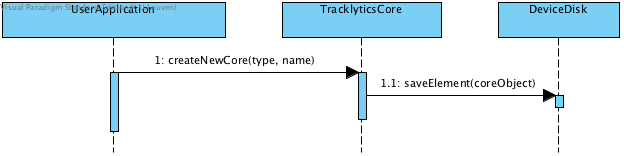
\includegraphics[scale=0.4]{Afbeeldingen/Architectuur/FlowDiagram1}
  \caption{Flow diagram 1.}
  \label{fig:flow1}
\end{figure}
\begin{figure}[!h]
  \centering
  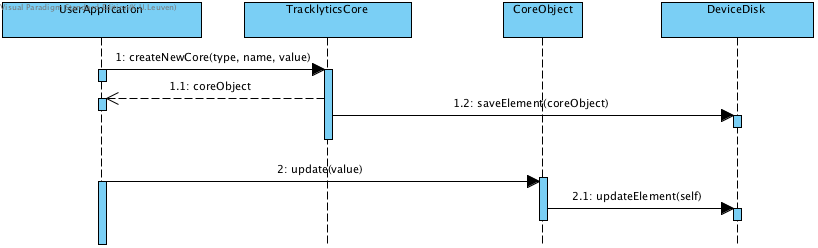
\includegraphics[scale=0.4]{Afbeeldingen/Architectuur/FlowDiagram2}
  \caption{Flow diagram 2.}
  \label{fig:flow2}
\end{figure}

Het monitoren van de gegevens van de applicatie kan opgesplitst worden in twee verschillende flows. \\

De eerste flow \ref{fig:flow1} toont de meest simpele flow. De developer geeft aan dat een bepaalde waarde gecollecteerd moet worden. De TracklyticsCore slaat deze informatie op op de schijf van het toestel van de gebruiker, zodat deze later verwerkt kan worden. De verwerking van de data wordt uitgelegd in de volgende sectie \ref{sec:VerzendenEnOpslaanVanGegevens}. Deze situatie is geldig in de gevallen dat de developer data voor een histogram of een gauge wil collecteren. De uitleg over deze componenten staat in het volgende hoofdstuk \ref{sec:Klassediagram}.\\

De tweede flow \ref{fig:flow2} toont een uitgebreidere flow van de vorige flow. Er wordt weer een bepaalde waarde gecollecteerd en deze wordt opgeslagen op de harde schijf van het toestel. Bij deze flow wordt een Core Object terug gegeven waar verdere acties mee mogelijk zijn. Deze acties worden gebundeld in de \texttt{update} call. Deze flow is geldig als de developer data voor een Counter, een Timer of een Meter wil collecteren. De uitleg over deze componenten en de acties die op deze componenten mogelijk zijn staan in het volgende hoofdstuk \ref{sec:Klassediagram} \\


\subsubsection{Verzenden en opslaan van de gegevens} \label{sec:VerzendenEnOpslaanVanGegevens}
In het volgende diagram \ref{fig:flow3} wordt getoond hoe het verzenden van de gegevens van het toestel naar de server in zijn werk gaat en hoe de gegevens worden opgeslagen in de database. 
\begin{figure}[!h]
  \centering
  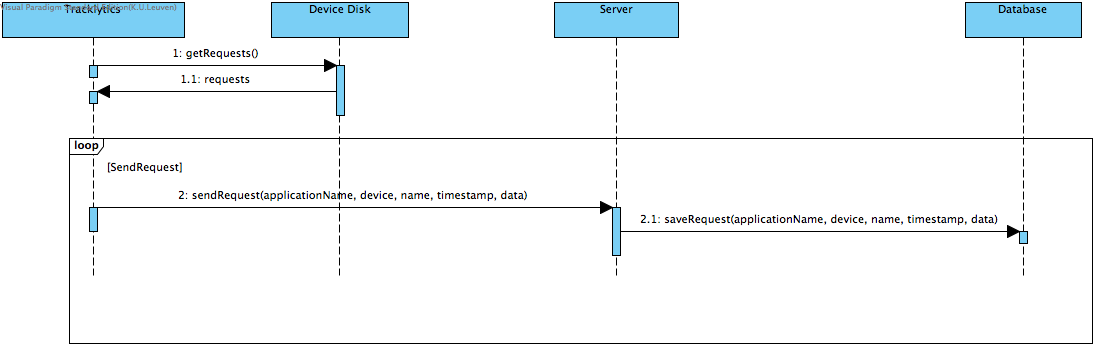
\includegraphics[scale=0.4]{Afbeeldingen/Architectuur/FlowDiagram3}
  \caption{Flow diagram 3.}
  \label{fig:flow3}
\end{figure}










%%% Local Variables: 
%%% mode: latex
%%% TeX-master: "masterproef"
%%% End: 
